%%%%%%%%%%%%%%%%%%%%%%%%%%%%%%%%%%%%%%%%%%%%%%%%%%%%%%%%%%%%%%%%%%
%%	  mmm  mmmmmm mm   m        m    m mmmmmm  mmmm				%%
%%	m"   " #      #"m  #        #    # #      #    #			%%
%%	#   mm #mmmmm # #m #        #    # #mmmmm "mmmm"			%%
%%	#    # #      #  # #  """   #    # #      	   #			%%
%%	 "mmm" #mmmmm #   ##        "mmmm" #mmmmm  #mmm"			%%
%%							      								%%
%%                                                              %%
%%                                                              %%
%%      Grundlagen der Elektrischen Netzwerke, UE               %%
%%      Gruppe 5, Team F                                        %%
%%      Authors: Severin Wolf, Maximilian Seidler.              %%
%%%%%%%%%%%%%%%%%%%%%%%%%%%%%%%%%%%%%%%%%%%%%%%%%%%%%%%%%%%%%%%%%%

\documentclass[a4paper]{article}

\usepackage{pstricks}
\usepackage{pst-circ}
\usepackage{pst-plot}
\usepackage{pstricks-add}
\usepackage[ngerman, english]{babel} 
\usepackage{amsmath}
\usepackage[latin1]{inputenc}
\usepackage{geometry}
\geometry{a4paper,left=3cm,right=2cm, top=2cm, bottom=2cm} 
\usepackage{graphicx}

\newpsobject{showgrid}{psgrid}{subgriddiv=1,griddots=10,gridlabels=0pt}
\psset{unit=1.0cm}
\psset{tensioncolor=blue}
\psset{tensionlabelcolor=blue}
\psset{intensitycolor=red}
\psset{intensitylabelcolor=red}

\setlength{\parindent}{0pt}
\usepackage{lipsum}

\newcommand\blfootnote[1]{%
	\begingroup
	\renewcommand\thefootnote{}\footnote{#1}%
	\addtocounter{footnote}{-1}%
	\endgroup
}
\begin{document}
	\pagestyle{empty} \enlargethispage*{25cm}\samepage{
		
		\vspace*{-3cm}
		\begin{center}
			\begin{minipage}[!h]{18cm}
				\hspace*{-0.9cm}
				\includegraphics[width=3.3cm]{./Figures/igte_logo}
				\begin{tabular}{p{10cm}}
					\vspace{1cm}
					\centering{
						\Large Institute of Fundamentals and Theory in
						Electrical Engineering\\
						Graz University of Technology\\
						~\\
						~\\}
				\end{tabular}
				\includegraphics[width=3.3cm]{./Figures/TUG_logo}
			\end{minipage}
			
			\vspace*{0.5cm}
			\Large
			\textbf{Fundamentals of electical circuits} \\
			\textbf{9. Homework}\\
			Multiports
			\vspace*{0.5cm}
			
			\large
			27 May 2021
	\end{center}}
	
	\vspace*{0.2cm}
	
	%%%%%%%%%%%%%%%%%%%%%%%%%%%%%%%%%%%%%%%%%%%%%%%%%%%%%%%%%%%%%%%%%%%%
	%%%%%%%%%%%%%%%%%%%%%%%%%%%%%%%%%%%%%%%%%%%%%%%%%%%%%%%%%%%%%%%%%%%%
	
	Consider the given circuit in figure~\ref{circuit}. There are three two-ports with passive elements connected in a cascade.

	\begin{enumerate}
		\item Determine the \textbf{Z}- and the \textbf{Y} set of parameters (independendly of each other), if possible. If it's not possible to calculate one of the parameter-sets, explain the reason briefly. Double-check your results by using the parameter conversion table ($[\underline{Z}] \rightarrow [\underline{Y}]$).
		
		\item Find the \textbf{A}-parameters (ABCD matrix) by using the parameter conversion table for all three two-port circuits.

		\item Calculate the voltage transfer-function $H(s) = \frac{U_{out}(s)}{U_{in}(s)}$ of the complete cascade connection. Bring the transfer-function in the following form: $H(s) = K\cdot \frac{s^2}{(1+\frac{s}{\omega_1})(1+\frac{s}{\omega_2})}$. Calculate the values of $K$, $\omega_1$ and $\omega_2$.

		\item Confirm the expression for the transfer-function in Matlab. \\
		Construct a Bode amplitude and phase-angle plot of the total transfer-function. 
		
		\item Simulate the circuit in LT-SPICE and compare the results for the transfer-function $H(s) = \frac{U_{out}(s)}{U_{in}(s)}$. 
	\end{enumerate}

	\subsection*{Values:}
$R_1=50~\Omega $, $R_2=2~k\Omega$, $R_3=600~\Omega$, $C=400 \mu F$, $L=20mH$.
\vspace{0.5cm}\\
\textbf{\textbf{Hint:} }
useful Matlab commands: \textbf{zpk, minreal, bode, zpkdata}.
 	
 	\begin{figure}[h!]
 		\centering
 		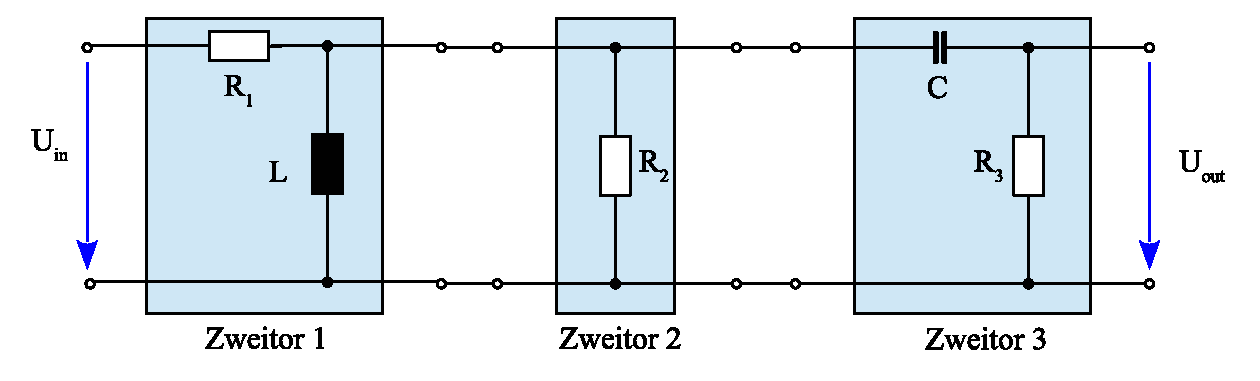
\includegraphics[width=1\textwidth]{./Figures/homework9_circuit.eps}
 		\caption{Teil 1 - cascade connection of three two-ports}
 		\label{circuit}
 	\end{figure}
\vspace{3.5cm}
 	\blfootnote{Deadline: 10 June 2021; \qquad Team I}
\end{document}